%% bare_conf.tex
%% V1.4b
%% 2015/08/26
%% by Michael Shell
%% See:
%% http://www.michaelshell.org/
%% for current contact information.
%%
%% This is a skeleton file demonstrating the use of IEEEtran.cls
%% (requires IEEEtran.cls version 1.8b or later) with an IEEE
%% conference paper.
%%
%% Support sites:
%% http://www.michaelshell.org/tex/ieeetran/
%% http://www.ctan.org/pkg/ieeetran
%% and
%% http://www.ieee.org/

%%*************************************************************************
%% Legal Notice:
%% This code is offered as-is without any warranty either expressed or
%% implied; without even the implied warranty of MERCHANTABILITY or
%% FITNESS FOR A PARTICULAR PURPOSE! 
%% User assumes all risk.
%% In no event shall the IEEE or any contributor to this code be liable for
%% any damages or losses, including, but not limited to, incidental,
%% consequential, or any other damages, resulting from the use or misuse
%% of any information contained here.
%%
%% All comments are the opinions of their respective authors and are not
%% necessarily endorsed by the IEEE.
%%
%% This work is distributed under the LaTeX Project Public License (LPPL)
%% ( http://www.latex-project.org/ ) version 1.3, and may be freely used,
%% distributed and modified. A copy of the LPPL, version 1.3, is included
%% in the base LaTeX documentation of all distributions of LaTeX released
%% 2003/12/01 or later.
%% Retain all contribution notices and credits.
%% ** Modified files should be clearly indicated as such, including  **
%% ** renaming them and changing author support contact information. **
%%*************************************************************************


% *** Authors should verify (and, if needed, correct) their LaTeX system  ***
% *** with the testflow diagnostic prior to trusting their LaTeX platform ***
% *** with production work. The IEEE's font choices and paper sizes can   ***
% *** trigger bugs that do not appear when using other class files.       ***                          ***
% The testflow support page is at:
% http://www.michaelshell.org/tex/testflow/



\documentclass[conference]{IEEEtran}
% Some Computer Society conferences also require the compsoc mode option,
% but others use the standard conference format.
%
% If IEEEtran.cls has not been installed into the LaTeX system files,
% manually specify the path to it like:
% \documentclass[conference]{../sty/IEEEtran}





% Some very useful LaTeX packages include:
% (uncomment the ones you want to load)


% *** MISC UTILITY PACKAGES ***
%
%\usepackage{ifpdf}
% Heiko Oberdiek's ifpdf.sty is very useful if you need conditional
% compilation based on whether the output is pdf or dvi.
% usage:
% \ifpdf
%   % pdf code
% \else
%   % dvi code
% \fi
% The latest version of ifpdf.sty can be obtained from:
% http://www.ctan.org/pkg/ifpdf
% Also, note that IEEEtran.cls V1.7 and later provides a builtin
% \ifCLASSINFOpdf conditional that works the same way.
% When switching from latex to pdflatex and vice-versa, the compiler may
% have to be run twice to clear warning/error messages.






% *** CITATION PACKAGES ***
%
\usepackage{cite}
% cite.sty was written by Donald Arseneau
% V1.6 and later of IEEEtran pre-defines the format of the cite.sty package
% \cite{} output to follow that of the IEEE. Loading the cite package will
% result in citation numbers being automatically sorted and properly
% "compressed/ranged". e.g., [1], [9], [2], [7], [5], [6] without using
% cite.sty will become [1], [2], [5]--[7], [9] using cite.sty. cite.sty's
% \cite will automatically add leading space, if needed. Use cite.sty's
% noadjust option (cite.sty V3.8 and later) if you want to turn this off
% such as if a citation ever needs to be enclosed in parenthesis.
% cite.sty is already installed on most LaTeX systems. Be sure and use
% version 5.0 (2009-03-20) and later if using hyperref.sty.
% The latest version can be obtained at:
% http://www.ctan.org/pkg/cite
% The documentation is contained in the cite.sty file itself.






% *** GRAPHICS RELATED PACKAGES ***
%
\ifCLASSINFOpdf
  % \usepackage[pdftex]{graphicx}
  % declare the path(s) where your graphic files are
  % \graphicspath{{../pdf/}{../jpeg/}}
  % and their extensions so you won't have to specify these with
  % every instance of \includegraphics
  % \DeclareGraphicsExtensions{.pdf,.jpeg,.png}
\else
  % or other class option (dvipsone, dvipdf, if not using dvips). graphicx
  % will default to the driver specified in the system graphics.cfg if no
  % driver is specified.
  % \usepackage[dvips]{graphicx}
  % declare the path(s) where your graphic files are
  % \graphicspath{{../eps/}}
  % and their extensions so you won't have to specify these with
  % every instance of \includegraphics
  % \DeclareGraphicsExtensions{.eps}
\fi
% graphicx was written by David Carlisle and Sebastian Rahtz. It is
% required if you want graphics, photos, etc. graphicx.sty is already
% installed on most LaTeX systems. The latest version and documentation
% can be obtained at: 
% http://www.ctan.org/pkg/graphicx
% Another good source of documentation is "Using Imported Graphics in
% LaTeX2e" by Keith Reckdahl which can be found at:
% http://www.ctan.org/pkg/epslatex
%
% latex, and pdflatex in dvi mode, support graphics in encapsulated
% postscript (.eps) format. pdflatex in pdf mode supports graphics
% in .pdf, .jpeg, .png and .mps (metapost) formats. Users should ensure
% that all non-photo figures use a vector format (.eps, .pdf, .mps) and
% not a bitmapped formats (.jpeg, .png). The IEEE frowns on bitmapped formats
% which can result in "jaggedy"/blurry rendering of lines and letters as
% well as large increases in file sizes.
%
% You can find documentation about the pdfTeX application at:
% http://www.tug.org/applications/pdftex
\usepackage[pdftex]{graphicx}





% *** MATH PACKAGES ***
%
\usepackage{amsmath}
\usepackage{amssymb}
\usepackage{amsthm}
% A popular package from the American Mathematical Society that provides
% many useful and powerful commands for dealing with mathematics.
%
% Note that the amsmath package sets \interdisplaylinepenalty to 10000
% thus preventing page breaks from occurring within multiline equations. Use:
%\interdisplaylinepenalty=2500
% after loading amsmath to restore such page breaks as IEEEtran.cls normally
% does. amsmath.sty is already installed on most LaTeX systems. The latest
% version and documentation can be obtained at:
% http://www.ctan.org/pkg/amsmath





% *** SPECIALIZED LIST PACKAGES ***
%
%\usepackage{algorithmic}
% algorithmic.sty was written by Peter Williams and Rogerio Brito.
% This package provides an algorithmic environment fo describing algorithms.
% You can use the algorithmic environment in-text or within a figure
% environment to provide for a floating algorithm. Do NOT use the algorithm
% floating environment provided by algorithm.sty (by the same authors) or
% algorithm2e.sty (by Christophe Fiorio) as the IEEE does not use dedicated
% algorithm float types and packages that provide these will not provide
% correct IEEE style captions. The latest version and documentation of
% algorithmic.sty can be obtained at:
% http://www.ctan.org/pkg/algorithms
% Also of interest may be the (relatively newer and more customizable)
% algorithmicx.sty package by Szasz Janos:
% http://www.ctan.org/pkg/algorithmicx
\usepackage[linesnumbered,ruled,vlined]{algorithm2e}




% *** ALIGNMENT PACKAGES ***
%
%\usepackage{array}
% Frank Mittelbach's and David Carlisle's array.sty patches and improves
% the standard LaTeX2e array and tabular environments to provide better
% appearance and additional user controls. As the default LaTeX2e table
% generation code is lacking to the point of almost being broken with
% respect to the quality of the end results, all users are strongly
% advised to use an enhanced (at the very least that provided by array.sty)
% set of table tools. array.sty is already installed on most systems. The
% latest version and documentation can be obtained at:
% http://www.ctan.org/pkg/array


% IEEEtran contains the IEEEeqnarray family of commands that can be used to
% generate multiline equations as well as matrices, tables, etc., of high
% quality.




% *** SUBFIGURE PACKAGES ***
%\ifCLASSOPTIONcompsoc
%  \usepackage[caption=false,font=normalsize,labelfont=sf,textfont=sf]{subfig}
%\else
%  \usepackage[caption=false,font=footnotesize]{subfig}
%\fi
% subfig.sty, written by Steven Douglas Cochran, is the modern replacement
% for subfigure.sty, the latter of which is no longer maintained and is
% incompatible with some LaTeX packages including fixltx2e. However,
% subfig.sty requires and automatically loads Axel Sommerfeldt's caption.sty
% which will override IEEEtran.cls' handling of captions and this will result
% in non-IEEE style figure/table captions. To prevent this problem, be sure
% and invoke subfig.sty's "caption=false" package option (available since
% subfig.sty version 1.3, 2005/06/28) as this is will preserve IEEEtran.cls
% handling of captions.
% Note that the Computer Society format requires a larger sans serif font
% than the serif footnote size font used in traditional IEEE formatting
% and thus the need to invoke different subfig.sty package options depending
% on whether compsoc mode has been enabled.
%
% The latest version and documentation of subfig.sty can be obtained at:
% http://www.ctan.org/pkg/subfig




% *** FLOAT PACKAGES ***
%
%\usepackage{fixltx2e}
% fixltx2e, the successor to the earlier fix2col.sty, was written by
% Frank Mittelbach and David Carlisle. This package corrects a few problems
% in the LaTeX2e kernel, the most notable of which is that in current
% LaTeX2e releases, the ordering of single and double column floats is not
% guaranteed to be preserved. Thus, an unpatched LaTeX2e can allow a
% single column figure to be placed prior to an earlier double column
% figure.
% Be aware that LaTeX2e kernels dated 2015 and later have fixltx2e.sty's
% corrections already built into the system in which case a warning will
% be issued if an attempt is made to load fixltx2e.sty as it is no longer
% needed.
% The latest version and documentation can be found at:
% http://www.ctan.org/pkg/fixltx2e


%\usepackage{stfloats}
% stfloats.sty was written by Sigitas Tolusis. This package gives LaTeX2e
% the ability to do double column floats at the bottom of the page as well
% as the top. (e.g., "\begin{figure*}[!b]" is not normally possible in
% LaTeX2e). It also provides a command:
%\fnbelowfloat
% to enable the placement of footnotes below bottom floats (the standard
% LaTeX2e kernel puts them above bottom floats). This is an invasive package
% which rewrites many portions of the LaTeX2e float routines. It may not work
% with other packages that modify the LaTeX2e float routines. The latest
% version and documentation can be obtained at:
% http://www.ctan.org/pkg/stfloats
% Do not use the stfloats baselinefloat ability as the IEEE does not allow
% \baselineskip to stretch. Authors submitting work to the IEEE should note
% that the IEEE rarely uses double column equations and that authors should try
% to avoid such use. Do not be tempted to use the cuted.sty or midfloat.sty
% packages (also by Sigitas Tolusis) as the IEEE does not format its papers in
% such ways.
% Do not attempt to use stfloats with fixltx2e as they are incompatible.
% Instead, use Morten Hogholm'a dblfloatfix which combines the features
% of both fixltx2e and stfloats:
%
% \usepackage{dblfloatfix}
% The latest version can be found at:
% http://www.ctan.org/pkg/dblfloatfix




% *** PDF, URL AND HYPERLINK PACKAGES ***
%
%\usepackage{url}
% url.sty was written by Donald Arseneau. It provides better support for
% handling and breaking URLs. url.sty is already installed on most LaTeX
% systems. The latest version and documentation can be obtained at:
% http://www.ctan.org/pkg/url
% Basically, \url{my_url_here}.




% *** Do not adjust lengths that control margins, column widths, etc. ***
% *** Do not use packages that alter fonts (such as pslatex).         ***
% There should be no need to do such things with IEEEtran.cls V1.6 and later.
% (Unless specifically asked to do so by the journal or conference you plan
% to submit to, of course. )


% correct bad hyphenation here
\hyphenation{op-tical net-works semi-conduc-tor}

\newtheorem{theorem}{Theorem}
\newenvironment{proof_}{{\indent \indent \it Proof:}}{\hfill $\blacksquare$\par}

\theoremstyle{definition}
\newtheorem{problem}{Problem}
\newtheorem*{GreedyApproach}{Greedy Approach for Problem 2}
\newtheorem*{GreedyApproacha}{Greedy Approaches for Problems 3 and 4}
\newtheorem{definition}{Definition}
% \newenvironment{definition}{}
\newtheorem{example}{Example}
\newtheorem*{Communication_in_Distributed_Algorithms}{Communication in Distributed Algorithms}
\newtheorem*{experiments}{Experiments}
\newtheorem*{Distributed_GA}{Distributed GA}
\newtheorem*{Generalizations_to_Arbitrary}{Generalizations to Arbitrary Sensing Regions, and
Coverage of an Area}
\newtheorem*{NP-Hardness of Approximating the SODkC Problem}{NP-Hardness of Approximating the SODkC Problem}

\newtheorem*{Greedy Algorithm (GA)}{Greedy Algorithm (GA)}
\newtheorem*{GA on the Running Example}{GA on the Running Example}
\newtheorem*{Performance Guarantee of GA}{Performance Guarantee of GA}
\begin{document}
%
% paper title
% Titles are generally capitalized except for words such as a, an, and, as,
% at, but, by, for, in, nor, of, on, or, the, to and up, which are usually
% not capitalized unless they are the first or last word of the title.
% Linebreaks \\ can be used within to get better formatting as desired.
% Do not put math or special symbols in the title.
% \title{Bare Demo of IEEEtran.cls\\ for IEEE Conferences}
\title{Selection and Orientation of Directional Sensors
\\for Coverage Maximization}


% author names and affiliations
% use a multiple column layout for up to three different
% affiliations
\author{\IEEEauthorblockN{Giordano Fusco and Himanshu Gupta}
\IEEEauthorblockA{Computer Science Department\\
Stony Brook University\\
Stony Brook, NY 11790\\
Email: \{fusco,hgupta\}@cs.sunysb.edu}
}

% conference papers do not typically use \thanks and this command
% is locked out in conference mode. If really needed, such as for
% the acknowledgment of grants, issue a \IEEEoverridecommandlockouts
% after \documentclass

% for over three affiliations, or if they all won't fit within the width
% of the page, use this alternative format:
% 
%\author{\IEEEauthorblockN{Michael Shell\IEEEauthorrefmark{1},
%Homer Simpson\IEEEauthorrefmark{2},
%James Kirk\IEEEauthorrefmark{3}, 
%Montgomery Scott\IEEEauthorrefmark{3} and
%Eldon Tyrell\IEEEauthorrefmark{4}}
%\IEEEauthorblockA{\IEEEauthorrefmark{1}School of Electrical and Computer Engineering\\
%Georgia Institute of Technology,
%Atlanta, Georgia 30332--0250\\ Email: see http://www.michaelshell.org/contact.html}
%\IEEEauthorblockA{\IEEEauthorrefmark{2}Twentieth Century Fox, Springfield, USA\\
%Email: homer@thesimpsons.com}
%\IEEEauthorblockA{\IEEEauthorrefmark{3}Starfleet Academy, San Francisco, California 96678-2391\\
%Telephone: (800) 555--1212, Fax: (888) 555--1212}
%\IEEEauthorblockA{\IEEEauthorrefmark{4}Tyrell Inc., 123 Replicant Street, Los Angeles, California 90210--4321}}




% use for special paper notices
%\IEEEspecialpapernotice{(Invited Paper)}




% make the title area
\maketitle

% As a general rule, do not put math, special symbols or citations
% in the abstract
\begin{abstract}
% The abstract goes here. 
Sensor nodes may be equipped with a “directional” sensing device (such as a camera) which senses a physical phenomenon in a certain direction depending on the chosen orientation. In this article, we address the problem of selection and orientation of such directional sensors with the objective of maximizing coverage area. Prior works on sensor coverage have largely focused on coverage with sensors that are associated with a \textit{unique} sensing region. In contrast, directional sensors have multiple sensing regions associated with them, and the orientation of the sensor determines the actual sensing region. Thus, the coverage problems in the context of directional sensors entails selection as well as orientation of sensors needed to activate in order to maximize/ensure coverage.

In this article, we address the problem of selecting a minimum number of sensors and assigning orientations such that the given area (or set of target points) is $k$-covered (i.e., each point is covered $k$ times). The above problem is NP-complete, and even NP-hard to approximate. Thus, we design a simple greedy algorithm that delivers a solution that $k$-covers at least half of the target points using at most $M\log(k|C|)$ sensors, where $|C|$ is the maximum number of target points covered by a sensor and $M$ is the minimum number of sensor required to $k$-cover all the given points. The above result holds for almost arbitrary sensing regions. We design a distributed implementation of the above algorithm, and study its performance through simulations. In addition to the above problem, we also look at other related coverage problems in the context of directional sensors, and design similar approximation algorithms for them.
\end{abstract}

% no keywords




% For peer review papers, you can put extra information on the cover
% page as needed:
% \ifCLASSOPTIONpeerreview
% \begin{center} \bfseries EDICS Category: 3-BBND \end{center}
% \fi
%
% For peerreview papers, this IEEEtran command inserts a page break and
% creates the second title. It will be ignored for other modes.
\IEEEpeerreviewmaketitle



\section{Introduction}
% I wish you the best of success.

Coverage problems have been extensively studied in the context of sensor networks (see for example \cite{1597223}, \cite{1146711}, \cite{936985}, \cite{10.1145/381677.381691}). The objective of sensor coverage problems is to minimize the number of active sensors, to conserve energy usage, while ensuring that the required region is sufficiently monitored by the active sensors. Most of the prior work has addressed the sensor coverage problem for single-orientation sensors, wherein each sensor is associated with a \emph{unique} sensing region which is typically modeled as a uniform disk centered at the sensor’s position. In this paper, we consider the sensor coverage problem in the context of “directional” sensors, such as cameras, whose sensing region depends upon the assigned orientation. Thus, the sensor coverage problem for directional sensors entails selection as well as orientation of active sensors to guarantee coverage.

In this article, we address the problem of selecting and orienting a minimum number of directional sensors to guarantee $k$-coverage of a given area or a set of target points (a point is $k$-covered if it is covered $k$ times). The above problem is trivially NP-complete, and we show that it is actually NP-hard even to approximate it within any bounded factor. Thus, we design a simple greedy algorithm that has the following performance guarantee. If there is a solution of size $M$ sensors that $k$-covers all the given target points, then our greedy algorithm delivers a solution that $k$-covers at least half of the target points (on average) using at most $M \log(k|C|)$ sensors, where $|C|$ is the maximum number of target points covered by a sensor. We also give a distributed implementation of the above greedy algorithm. In our experiments over dense random networks and target points, the greedy algorithm performs very well and selects only about $25\%$ more sensors than the theoretical minimum.

In addition to the above problem of selection and orientation of directional sensors, we also present approximation algorithms for the following related problems
on directional sensors: (\romannumeral 1) Orient all the given sensors in order to maximize coverage, (\romannumeral 2) Place and orient a minimum number of sensors in order to cover the given
area, (\romannumeral 3) Place and orient the given number of sensors
to maximize the area covered.

\noindent\textbf{Paper Organization.} The rest of the paper is organized as follow. Section \uppercase\expandafter{\romannumeral 2} contains detailed discussion about related work. The $k$-coverage problem is introduced in Section \uppercase\expandafter{\romannumeral 3}. The greedy algorithm is presented in Section \uppercase\expandafter{\romannumeral 4}. We discuss related problems in Section \uppercase\expandafter{\romannumeral 5}, and our experimental results in section \uppercase\expandafter{\romannumeral 6}.

\section{Related work}
In the recent years, there has been a lot of research done \cite{1146711}, \cite{936985}, \cite{1181406}, [1] to address the coverage problem in sensor networks. In particular, Slijepcevic and Potkonjakthe [3] design a centralized heuristic to select mutually exclusive sensor covers that independently cover the network region. In [2], Charkrabarty et al. investigate linear programming techniques to optimally place a set of sensors on a sensor field for a complete coverage of the field. In \cite{1208944}, Shakkottai et al. consider an unreliable sensor network, and derive necessary and sufficient conditions for the coverage of the region and connectivity of the network with high probability. Recently, Hefeeda and Bagheri \cite{4215866} extended the well-known $\varepsilon$-nets technique to solve the problem of $k$-covering the given sensor locations. In one of our prior works [1], we designed a greedy approximation algorithm that delivers a connected sensor-cover within a logarithmic factor of the optimal solution; this work was later generalized to $k$-coverage in \cite{1401672}.

Two closely related problems to the sensor-coverage problem are the art-gallery and hitting-set problems. The art-gallery problem (see \cite{10.5555/40599} for a survey) is to place a minimum number of guards in a polygon so that each point in the polygon is visible from at least one of the guards. Guards may be looked upon as cameras with infinite range (angular and distance). The hitting-set problem is a “dual” of the set-cover problem. In both set-cover and hitting-set problems, we are given sets and elements. While in set-cover the goal is to select the minimum number of sets to cover all elements/points, in hitting-set the goal is to select a subset of elements/points such that each set is hit. The classical result for set cover \cite{10.5555/580470} gives a $O(\log |C|)$ approximation, where $|C|$ is the size of the largest set. Bronnimann and Goodrich \cite{10.1007/BF02570718} were the first to use the $\varepsilon$-net technique \cite{10.1007/BF02187876} to solve the hitting-set problem and hence the set-cover with an $O(\log M)$ approximation, where $M$ is the size of the optimal solution.

All of the above works are for single-orientation sensors, wherein each sensor is associated with a unique sensing region, typically a uniform disk. In contrast, in this article, we consider $k$-coverage of a region using directional sensors, wherein each sensor is associated with a set of sensing regions, among which one is chosen based on the selected orientation. To the best of our knowledge, there are only two works, \cite{article} and \cite{10.1145/1178782.1178800}, that have addressed coverage problems for directional sensors. In particular, for the specific case of cameras (with directional-cones as sensing regions), Ai
and Abouzeid [13] propose a greedy heuristic (without any performance guarantee) to orient the given cameras in order to maximize 1-coverage (i.e., Problem 2 of Section \uppercase\expandafter{\romannumeral 5} of this article). In another work, H\"orster and Lienhart [14] address a number of camera-coverage problems, and design heuristics or exponential-time algorithms for each one of them. In this article, we address similar coverage problems for more general directional sensors, and present approximation algorithms for them.


\begin{figure}[t]
    \centering
    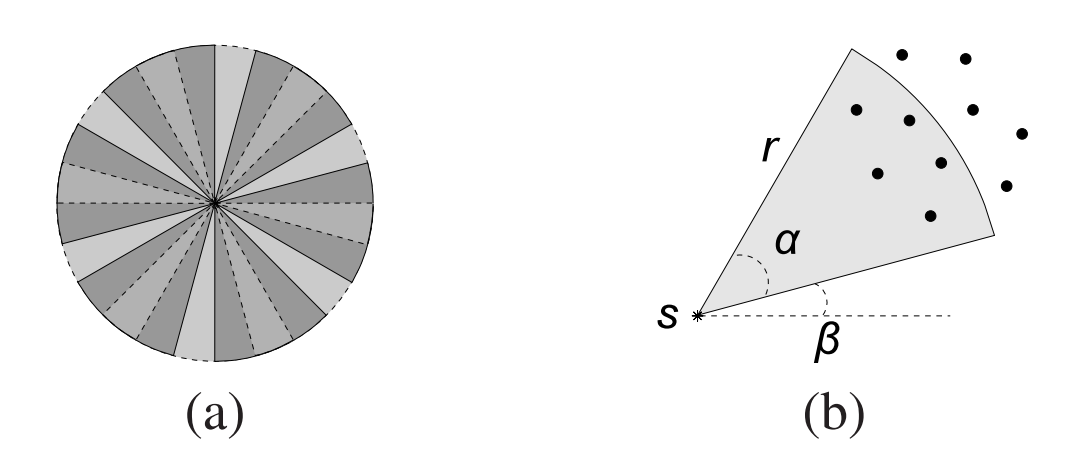
\includegraphics[width=0.8\columnwidth]{1.png}
    \caption{(a) Sensing regions associated with a d-sensor. (b) A selected selected sensing region corresponding to the orientation $\beta$, and given target points.}
    \label{fig:enter-label}
\end{figure}

In the early years, as the effective charging range of WCVs is quite finite (typically as low as a few meters in practice) and sensors are physically isolated from each other, WCVs need to move to sensors close to charge the sensors. Most works are based on such a scenario [12], [13]. The challenges of mobile charging in Wireless Rechargeable Sensor Networks include energy and time limitations of the Wireless Charging Vehicles, energy overheads caused by their travelling, and remote locations of some sensors.

\section{Problem Formulation}
We start with formally defining a directional-sensor (d-sensor, in short) and the problem of selection and orientation of d-sensors to guarantee coverage of a given area. Informally, a d-sensor is a sensor associated with multiple sensing regions, out of which only one is active, depending on the orientation assigned to the d-sensor. The simplest example of a d-sensor is a camera – which senses a cone of a certain radius $r$ and angle $\alpha$, depending on the angle of orientation $\beta$. See Figure 1. \textbf{\emph{For the sake of simplicity and clarity}}, we assume the d-sensors to be like cameras, i.e., the associated sensing regions to be uniform sized cones (as in \cite{10.1007/11599463_70} and \cite{4068136}). \textbf{\emph{Our algorithms and their performance guarantees generalize to arbitrary sensing regions, as discussed later.}}

\begin{figure}
    \centering
    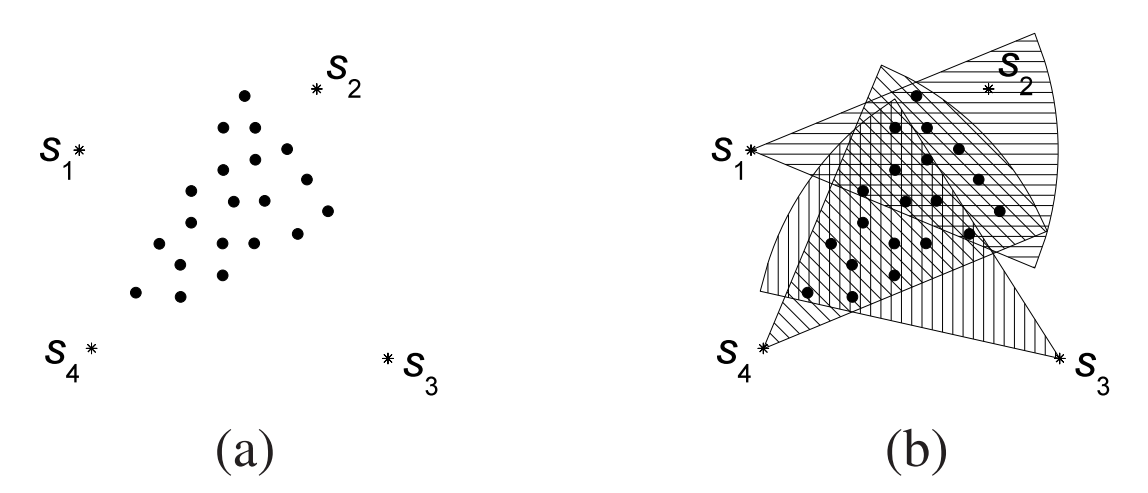
\includegraphics[width=0.8\columnwidth]{2.png}
    \caption{Illustrating the SODkC problem. Suppose we are given 4 d-sensors of centers $s_1,\dots,s_4$ and 20 points as in (a). Each d-sensor has associated many cone-shaped sensing regions as in Figure 1. The problem is to select the minimum number of d-sensor and orient them to $k$-cover all points. A possible solution for $k = 2$ is shown in (b), where 3 sensor suffice to 2-cover all points.
}
    \label{fig:enter-label}
\end{figure}

% \textbf{Definition 1.} 
\begin{definition}
(Directional Sensor (d-sensor); Orientation) We model a \textit{d-sensor} as a sensor associated with multiple (actually infinite) sensing regions in the given 2D plane. Each associated sensing region is a 2D cone of uniform radius $r$ and coverage angle $\alpha$, centered at the d-sensor’s position/location $s$. See Figure 1(a). The $orientation$ of a d-sensor is an angle used to select \textbf{one} of its associated sensing region. For instance, in Figure 1(b), the orientation is $\beta$, and the shaded region is the selected sensing region.$\hfill\square$
\end{definition}

\begin{definition}
(Target Points) \textit{Target points} are given points in the 2D plane that we wish to cover using the d-sensors.$\hfill\square$
\end{definition}

% \textbf{Problem 1.}
\begin{problem}
(Selecting and Orienting d-sensors for $k$-coverage (\textbf{SODkC})) Given a set of d-sensors with fixed positions and a set of target points, select the minimum number of d-sensors and their assigned orientations, such that each target point is covered (is contained in the selected sensing region) by at least $k$ of the selected d-sensors.
\end{problem}

For simplicity, we have defined the above SODkC problem’s objective as coverage of a set of given target \textit{points}. However, as discussed later, our designed algorithms and techniques easily generalize to the problem of covering a given area.

% \textbf{Example 1.} 
\begin{example}    
Suppose we are given 4 sensors and 20 points as in Figure 2(a), and we want to select the minimum number of d-sensor and orient them to 2-cover all points. In this particular example, 2 sensors are not enough to 2-cover all points. Instead, 3 sensors suffices, as shown in Figure 2(b).$\hfill\square$
\end{example}

% \textbf{NP-Hardness of Approximating the SODkC Problem.}
\begin{NP-Hardness of Approximating the SODkC Problem}
We now show that it is NP-hard to approximate the above SODkC problem, by first showing the NP-completeness of the corresonding decision problem: Given a set of dsensors with fixed locations, is there a way to orient the d-sensors so as to cover the given target points? This decision problem is NP-complete, as shown below using a reduction from 3-SAT.
% \end{NP-Hardness of Approximating the SODkC Problem}

\begin{algorithm}[t]
    \caption{Greedy Algorithm (GA) -Selecting and orienting d-sensors for $k$-coverage}
    \While{\textnormal{there are targets not $k$-covered yet \textbf{and} there are d-sensors not yet oriented}}{Select a d-sensor (that has not been selected yet) and an orientation pair that covers the most number of target points not yet $k$-covered;}
\end{algorithm}

\noindent\underline{Reducing 3-SAT to the Decision Problem of SODkC.} Given an instance of 3-SAT, i.e., a disjunction of conjunctive 3-literal clauses, we create a target point for each clause, a d-sensor for each variable, and two sensing regions (called positive and negative) for each sensor. The positive sensing region covers all the target points corresponding to clauses that contain the positive literal of the variable, and the negative sensing region covers all the target points corresponding to clauses that contain the negative literal of the variable. It is easy to see that the above reduction is a valid Karp-reduction from 3-SAT to our decision problem. Thus, the decision problem of SODkC is NP-complete.
\end{NP-Hardness of Approximating the SODkC Problem}


Now, if it were possible to approximate (within any bounded factor) the SODkC problem in polynomial time, then we can solve the decision problem by just using the approximation algorithm. Note that the approximate algorithm returns a bounded solution iff there is some way (an optimal solution) to orient the d-sensors to cover the target points. Thus, it is NP-hard to approximate the SODkC problem.

% \begin{figure}
%     \centering
%     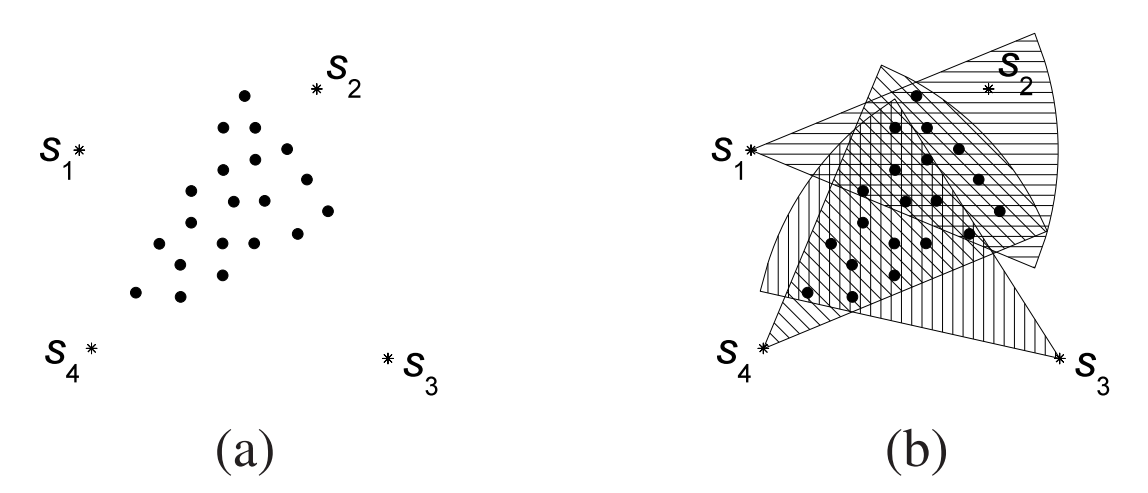
\includegraphics[width=0.8\columnwidth]{2.png}
%     \caption{Illustrating the SODkC problem. Suppose we are given 4 d-sensors of centers $s_1,\dots,s_4$ and 20 points as in (a). Each d-sensor has associated many cone-shaped sensing regions as in Figure 1. The problem is to select the minimum number of d-sensor and orient them to $k$-cover all points. A possible solution for $k = 2$ is shown in (b), where 3 sensor suffice to 2-cover all points.
% }
%     \label{fig:enter-label}
% \end{figure}

\section{GA: Greedy Algorithm}
In this section, we present our Greedy Algorithm, for the SODkC problem. We present the performance guarantee of the algorithm, and discuss its generalizations.

% \textbf{Greedy Algorithm (GA).} 
\begin{Greedy Algorithm (GA)}
Greedy Algorithm works in iterations. At each iteration, it considers all d-sensors that have not been yet selected in previous iterations. For each such d-sensor, it considers all its possible orientations, and picks the (d-sensor, orientation) pair that covers the largest number of target points that have not been yet $k$-covered (by previously selected dsensors). The algorithm terminates when all the target points are k-covered (i.e., covered by at least $k$ selected d-sensors). See Algorithm 1. Note that in the above algorithm, the selection of a d-sensor and the assignment of its orientation is permanent (i.e., not altered in later iterations). Morever, not all d-sensors are selected; the d-sensors not selected by the algorithm are essentially kept inactive to save energy.
\end{Greedy Algorithm (GA)}

% \textbf{GA on the Running Example.} 
\begin{GA on the Running Example}
Consider the example in Figure 2. GA selects and orients $s_4$ first, because it can cover the highest number of points (20 in this case). Then it selects and orients $s_3$ because it can cover 15 points for the 2nd time (note that $s_2$ could also cover 15 points, but ties are resolved arbitrarily). Finally, $s_1$ is selected to 2-cover the remaining 5 points.
\end{GA on the Running Example}

% \textbf{Performance Guarantee of GA.} 
\begin{Performance Guarantee of GA}
Note that GA’s solution may not $k$-cover all the given target points, even if there is some solution that does it. See Figure 3. The problem to determine whether there is a solution (i.e., a way to orient a set of given d-sensors) that $k$-covers the given target points is NP-complete as shown above. In the below theorem, we prove that if there is some solution that $k$-covers the set of given target points, then GA yields a solution which has a “benefit” of half the optimal and uses at most $O(\log_{}|C|)$ times the optimal number of d-sensors.
\end{Performance Guarantee of GA}

We now define a concept of benefit of an arbitrary set of sensing regions, at a given stage of GA, which will be used in stating and proving the performance guarantee of GA.

\begin{figure}
    \centering
    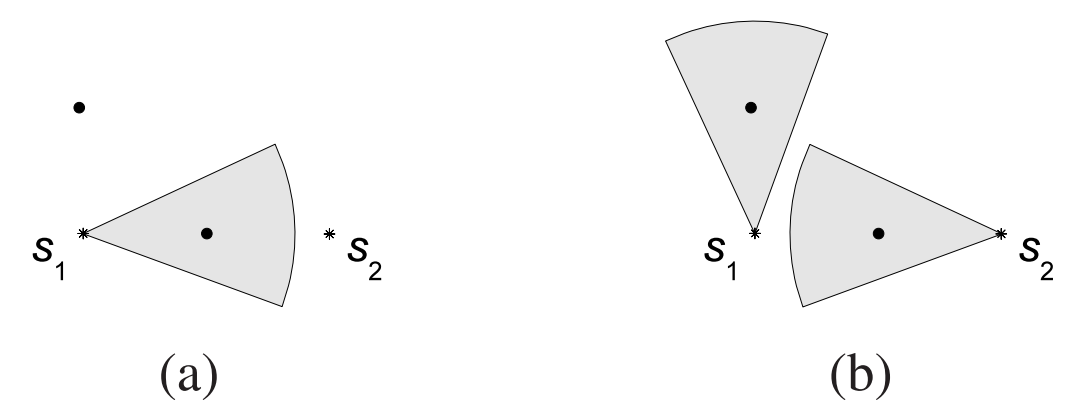
\includegraphics[width=0.8\columnwidth]{3.png}
    \caption{Counterexample that GA may not find the optimal solution. GA might orient sensor $s_1$ towards the target point in the middle leaving the other point uncovered as in (a), while it is possible to
cover both points as in (b).}
    \label{fig:enter-label}
\end{figure}

% \textbf{Definition 3.} 
\begin{definition}
(Benefit of a Set of Sensing Regions) Consider a given stage of GA, wherein GA has already selected and oriented some set of d-sensors. Informally, the \textit{benefit} of a \textit{sensing region} is the number of target points that it covers that are not yet \textit{k-covered} by GA. Similarly, the \textit{benefit} of a set $\mathcal{Q}$ of \textit{sensing regions} is the “additional number of times” the set $\mathcal{Q}$ covers the uncovered (not yet $k$-covered by GA) target points. More formally, let $\mathcal{G}$ be the set of sensing regions already selected by the greedy algorithm. Also, let $T'$ denote the set of yet uncovered (by GA) target points, i.e.,
\begin{equation*}
    \begin{split}
        T' = \{x | &\text{number of sensing regions selected by GA} \\
        &\text{that cover $x$ is less than $k$} \}. 
    \end{split}
\end{equation*}
The benefit of $\mathcal{Q}$ is defined as
\begin{equation*}
    \begin{split}
        \sum_{x \in T'} &\min \Big \{ (\text{number of sensing regions in $\mathcal{Q}$ that cover $x$),} \\
        & k - \text{(number of sensing regions in $\mathcal{G}$ that cover $x$}) \Big \}.\hfill\square
    \end{split}
\end{equation*}
\end{definition}

\begin{theorem}
Consider a given instance of SODkC problem. If there exists a solution that provides $k$-coverage to the given set of target points, then GA returns a solution that has a benefit of at least $k|T|/2$ and uses at most $O(\ln k|C|)$ times the number of d-sensors used by an optimal algorithm. Here, $n$ is the total number of d-sensors, $|T|$ is the number of target points, and $|C|$ is the maximum number of target points covered by a sensing region. Also, GA can be implemented to run in $O(kn|T|^2 \log n|T|)$ time.
\end{theorem}

\begin{proof_}
Let $n_g$ be the number of d-sensors selected (and oriented) by GA; let us number these d-sensors as $1, 2,\dots,n_g$ in the order they were selected by GA. Also, let $g_i$ be the benefit of the sensing region chosen in the $i^{th}$ step of GA.
\end{proof_}

Consider the stage when GA has selected (and oriented) $1, 2,\dots,j$ d-sensors. In the next paragraph, we will prove the \textbf{claim} that at this stage (when GA has already selected and oriented 1 to $j$ d-sensors), there is an orientation of some unselected d-sensor that covers at least $(k|T| - 2\sum_{i=1}^j g_i)/n_{opt}$ uncovered (not yet $k$-covered) target points, where $n_{opt}$ is the number of d-sensors selected by an optimal algorithm. Since GA picks the best (d-sensor, orientation) pair in the following iteration, the above claim implies that
\begin{equation*}
    g_{j + 1} \geq \frac{1}{n_{opt}} \Bigg(k|T| - 2\sum_{i=1}^j g_i \Bigg)
\end{equation*}
Now, we can show by induction that
\begin{equation*}
    (k|T| - 2\sum_{i=1}^j g_i) \leq k|T| \Bigg(1 -\frac{2}{n_{opt}}\Bigg)^j.
\end{equation*}
Thus, when $j = n_{opt}/2 \ln(k|T|/n_{opt})$, we have $(k|T| - 2\sum_{i=1}^j g_i) < n_{opt}$. Finally, observing that $nopt|C| \leq k|T|$ and that GA will continue until $(k|T| - 2\sum_{i=1}^j g_i)$ is zero, we see that when GA terminates, it has a benefit of at least $k|T|/2$ and uses at most $O(\ln k|C|)$ d-sensors.

% Proving the Claim.
\noindent\underline{Proving the Claim.} Consider the stage when GA has selected (and oriented) $1, 2,\dots,j$ d-sensors. Let us consider the sensing regions selected by the optimal algorithm at this stage. Note that some of these sensing regions may belong to the 1 to $j$ d-sensors already selected by GA, and may even be same as the one selected by GA. See Figure 4(a). We make the following two observations about the benefit of sensing regions selected by the optimal algorithm.

\begin{itemize}
    \item The benefit of the $n_{opt}$ optimal sensing regions is at least $(k|T| - \sum_{i=1}^j g_i)$ at this stage of GA.
    \item The benefit of the optimal sensing regions excluding the ones that belong to the 1 to $j$ d-sensors (which have been already selected by GA at this stage) is at least
    \begin{equation*}
        (k|T| - \sum_{i=1}^j 2g_i).
    \end{equation*}
    Note that number of sensing regions constituting the above benefit is at most $(n_{opt} - j)$. See Figure 4(b). The above observation is true because the benefit of an optimal sensing region $o_i$ associated with an $i$ d-sensor at this stage is at most the benefit of $o_i$ at the stage when $i$ d-sensor was selected by GA. The latter is at most $g_i$, the benefit of the sensing region chosen by GA in the $i^{th}$ iteration.
\end{itemize}
Finally, by the pigeon-hole principle, there must be at least one unselected d-sensor whose benefit at this stage is at least $(k|T| - 2\sum_{i=1}^jg_i)/(n_{opt} - j) > (k|T| - 2\sum_{i=1}^j g_i)/n_{opt}$.

\begin{figure}
    \centering
    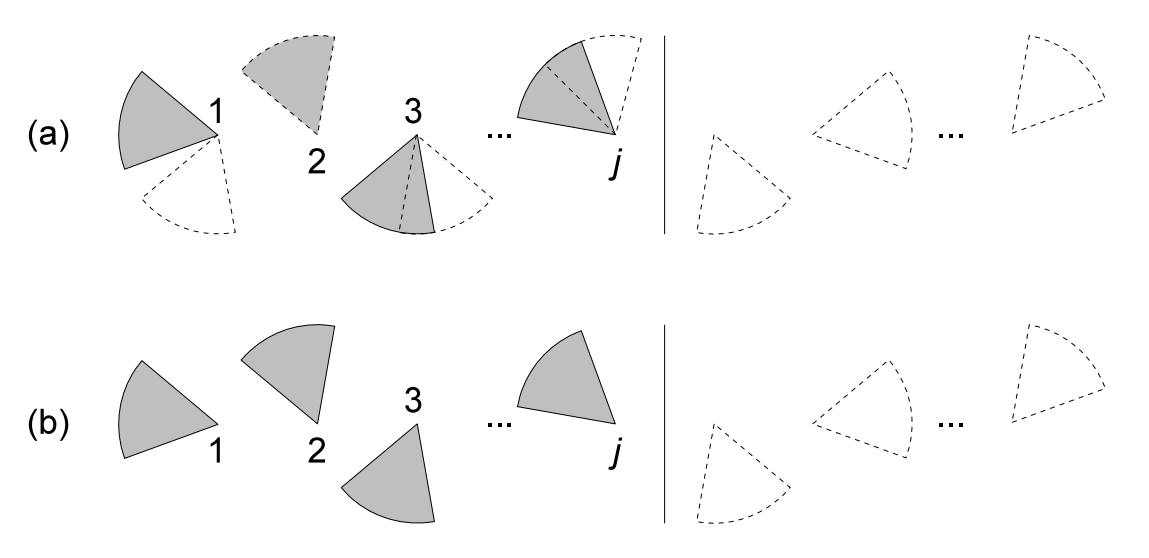
\includegraphics[width=0.8\columnwidth]{4.png}
    \caption{The dotted cones are sensing regions picked by the optimal algorithm, and the shaded ones are those picked by GA. (a) The optimal sensing regions at the stage when GA has selected and oriented $1, 2,\dots,j$ d-sensors. (b) The optimal sensing regions
excluding the ones that belong to $1, 2,\dots,j$ d-sensors.
}
    \label{fig:enter-label}
\end{figure}

\noindent\underline{Running Time.} The algorithm can be implemented efficiently by keeping a priority queue of d-sensors’ orientations based on the number of uncovered (not yet $k$-covered) targets that each d-sensor’s orientation can cover. Note that the total number “relevant” orientations for a d-sensor is at most $|T|$, and thus, the size of the priority queue is at most $n|T|$. The loop is executed at most $k|T|$ times. In each iteration, extracting the best (d-sensor, orientation) pair from the queue requires $O(\log n|T|)$ time and updating the priorities of elements takes at most $O(n|T| \log n|T|)$ time (since there are at most $n|T|$ elements and each update takes at most $O(\log n|T|)$ time).\hfill $\blacksquare$

\begin{algorithm}
    \caption{Distributed GA (algorithm of each d-sensor) — Selecting and orienting d-sensors for $k$-coverage}

    $status = $ unselected\;
    \While{\textnormal{there are owned target points that are not $k$-covered}}{
    pick one such owned target point $t$\;
    send a {\fontfamily{qcr}\selectfont benefit-enquiry} message to neighboring {\fontfamily{qcr}\selectfont unselected} d-sensors that cover $t$, asking their maximum benefit if selected and oriented to cover $t$\;
    \lIf{\textnormal{there are no answers}}{ \Return{\fontfamily{qcr}\selectfont failure}}
    \lElse{select the d-sensor with maximum benefit and send it a {\fontfamily{qcr}\selectfont selection-request}}
    }
    \While{true}{
    \If{status $==$ \textnormal{\fontfamily{qcr}\selectfont unselected}}{
    \ForEach{\textnormal{\fontfamily{qcr}\selectfont benefit-enquiry}}{determine the best orientation to cover the given $t$, and inform the requesting d-sender of the benefit\;}
    }
    }
    \While{true}{
    \If{status $==$ \textnormal{{\fontfamily{qcr}\selectfont unselected} \textbf{and} there is at least one {\fontfamily{qcr}\selectfont selection-request}}}{
    satisfy the request that will result in maximum benefit\;
    $status =$ {\fontfamily{qcr}\selectfont selected}\;
    Inform the near-by d-sensors (that cover a common target point) of the selection and orientation\;
    }
    }
    
\end{algorithm}

% Generalizations to Arbitrary Sensing Regions, and Coverage of an Area. 
\begin{Generalizations_to_Arbitrary}
The Greedy Algorithm (GA) easily extends (along with its performance guarantee) to d-sensors with sensing regions of arbitrary shape, as long as the the sensing regions are compact.\footnote{A region is compact if it is closed and connected. In particular, this is true if each region covers a finite number of points.} For such d-sensors with arbitrary sensing regions, the concept of orientation may be defined as some way of identifying the different sensing regions. Note that the proof of the above Theorem 1 is independent of the shapes of the sensing regions.
\end{Generalizations_to_Arbitrary}

Similarly, GA can also be used to $k$-cover a given area, rather than a given set of target points (as required by the formulation of SODkC problem). Essentially, coverage of an area requires dividing the given area into “subregions” as in our previous work [1]; a subregion is defined as a set of points in the plane that are covered by the \textit{same} set of sensing regions. The number of such subregions can be shown to be polynomial in the total number of cone-shaped sensing regions in the system.

Based on the above, we define the benefit of a sensing region as the number of number of uncovered subregions contained in the sensing-region. The Greedy Algorithm can then be used without any other modification, and the performance guarantees still hold.

% \begin{figure}
%     \centering
%     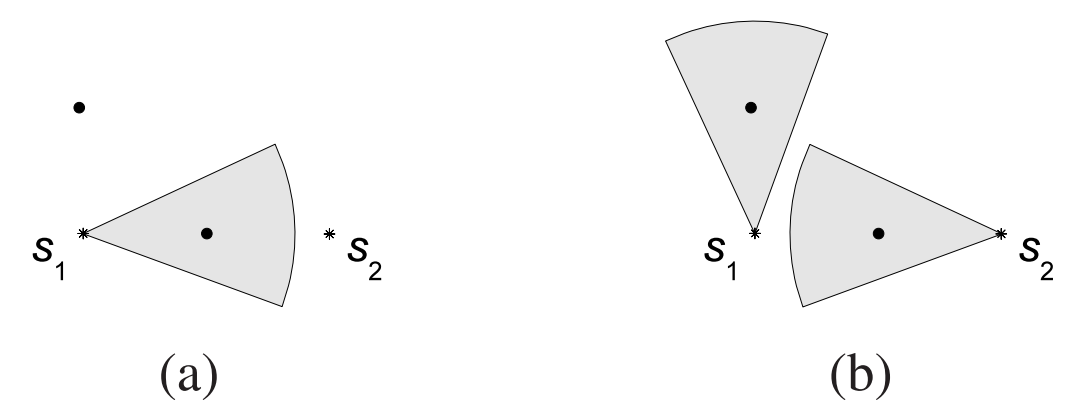
\includegraphics[width=0.8\columnwidth]{3.png}
%     \caption{Counterexample that GA may not find the optimal solution. GA might orient sensor $s_1$ towards the target point in the middle leaving the other point uncovered as in (a), while it is possible to
% cover both points as in (b).}
%     \label{fig:enter-label}
% \end{figure}

% Distributed GA.
\begin{Distributed_GA}
In a distributed environment, \textit{conceptually}, each yet-uncovered target point increases its coverage by selecting and orienting a d-sensor that covers it and has the highest benefit at that stage. The above process continues until all target points are $k$-covered. To facilitate the above, a target point (or a subregion) is “owned” by the highest-ID d-sensor that can cover it using one of its sensing regions. Thus, each d-sensor ensures coverage of the target points owned by it, through selection and orientation of near-by d-sensors. See Algorithm 2, for a pseudo-code of the distributed algorithm.
\end{Distributed_GA}

\section{Related Problems}
In this section, we address problems similar to our SODkC problem that were presented in [14], in the context of coverage by placing and/or orienting cameras. We show that our GA can be modified to yield approximation algorithms for each of these related problems.

\begin{problem}
    (Orienting all d-sensors for Maximizing
Coverage) Given a set of d-sensors with fixed positions
and a set of target points, orient all d-sensors so as to
cover the maximum number of target points.
\end{problem}

The above problem is also addressed in [13], wherein the authors present a greedy heuristic (different than ours) without a provable performance guarantee. In contrast, we present below a greedy approach with a constant-factor approximation.

\begin{GreedyApproach}
The above problem can be solved using greedy approach similar to the GA, with the only difference that we continue to select and orient d-sensors until all the d-sensors have been oriented. At each stage, we pick a (d-sensor, orientation) pair that has the maximum benefit at that stage. See Algorithm 3. The running time of the algorithm is same as GA, i.e., $O(kn|T|^2 \log n|T|)$, but in this case, we get constant-factor approximation as shown in the following theorem.
\end{GreedyApproach}

\begin{algorithm}[t]
    \caption{Orienting all d-sensors for max-coverage}
    \While{\textnormal{there are d-sensors not oriented yet}}{Select a d-sensor (that has not been selected yet) and an orientation pair that covers the most number of target points not yet covered\;}
\end{algorithm}

\begin{theorem}
    The greedy approach (as described above) yields a 0.43-approximate solution to Problem 2.
\end{theorem}

\begin{proof_}
    Let $M$ be the \textit{number of target points} covered by the optimal solution. This proof proceeds in a similar way as the proof of Theorem 1, and yields the below equation.
    \begin{equation*}
        g_{j+1} \geq \frac{1}{n} \Bigg(M-2\sum_{i=1}^j g_i \Bigg)
    \end{equation*}
    Above, $g_{j+1}$ is the benefit of the sensing-region chosen in the $j^{th}$ step of the greedy approach. By induction, we can show that
    \begin{equation*}
        (M - 2\sum_i g_{i+1}) \leq M \bigg(1 - \frac{2}{n} \bigg)^j,
    \end{equation*}
    which yields
    \begin{equation*}
        \frac{\sum_{i=1}^n g_i}{M} \geq \frac{1}{2} \bigg(1-\bigg(1-\frac{2}{n}\bigg)^n\bigg) \geq \frac{1}{2} \bigg(1-\frac{1}{e^2}\bigg)=0.43.
    \end{equation*}
\end{proof_}

\begin{problem}
    (Placing and Orienting d-sensors for MinCost Coverage) Given a polygon $P$ and a set of d-sensors
along with their \textit{costs} and associated sensing regions.
Cover a given percentage $p$ of the area of the polygon
$P$, by placing and orienting a minimum cost subset of
given d-sensors.
\end{problem}

\begin{problem}
(Placing and Orienting d-sensors for MaxCoverage) Given a polygon $P$ and a set of d-sensors along with their \textit{costs} and associated sensing regions. Cover a maximum percentage of $P$’s area, by placing and orienting a subset of given d-sensors whose cost is less than the given budget $B$.
\end{problem}

\begin{GreedyApproacha}
We use greedy approaches similar to GA to solve Problems 3 and 4. Essentially, at each stage, we pick the best (d-sensor, position, orientation) triplet that gives the highest ratio of \textit{area-covered/cost}. See Algorithms 4 and 5. For a given d-sensor and orientation, we can find its best placement using the algorithm in [17]. The result in [17] is for placement of “360-degree guards,” but their result can be easily extended for arbitrary closed and connected sensing-regions, provided that VC-dimension (defined below) remains bounded. The use of their approach allows us to finds a position for a given d-sensor and orientation that covers $(1 - \delta)$ times the optimal area possible in $O((n^2 l^2/\delta^4) \log^3(l/\delta))$ time, where $l$ is the size of the given polygon. We start by stating the time complexity, and then we will prove the approximation
factors of the above greedy approaches.
\end{GreedyApproacha}

\begin{algorithm}
\caption{Placing and orienting d-sensors for min-cost
coverage}    
\While{\textnormal{$P$ is not covered for at least $p$ percent}}{
$best\_d\_sensor = null$\;
\ForEach{\textnormal{d-sensor type}}{
\ForEach{\textnormal{discretized orientation}}{
run the algorithm in \cite{10.5555/982792.982954} to find the best position for this d-sensor type and orientation\;
\If{\textnormal{this combination gives a higher ratio of (area covered/d-sensor cost) than $best\_d\_sensor$}}{store this combination in $best\_d\_sensor$\;}
keep $best\_d\_sensor$\;
remove the area covered by $best\_d\_sensor$ from the polygon to cover\;}
}
}
\end{algorithm}

\begin{theorem}
The above described greedy approaches for Problems 3 and 4 run in time $O(\tau nuR)$ time, where $\tau$ is the number of different d-sensors types, $u$ is the number of discretized d-sensor’s orientations, $n$ is the total number of d-sensor, and $R$ is the running time of the algorithm in [17]. In particular, $R = O((n^2 l^2 /\delta^4) \log^3(l/\delta))$ where $l$ is the number of edges of the polygon $P$ and $\delta > 0$ is the parameter that affects the precision of the result.
\end{theorem}

Before proving the approximation factors, we need to introduce the concept of Vapnik-\v{C}ervonenkis (VC) dimension. The VC-dimension is defined in terms of set shattering, as follows.

\begin{definition}
(VC dimension) A set $X$ is \textit{shattered} by $\mathcal{C}$ if for each $Y \subseteq X$, there exists a set $S \in \mathcal{C}$ such that $X \cap S = Y$. The \textit{VC dimension} is the cardinality of the
largest set that can be shattered by $\mathcal{C}$. \hfill $\square$
\end{definition}

In our case, the VC dimension of the set of d-sensor’s sensing regions is at most 23, as given by Valtr theorem \cite{Valtr1998GuardingGW}:

\begin{theorem}
If $X \subset \mathbb{R}^2$ is compact and simply connected, then VC-dimension of the system $V(X) = \{V (x) | x \in X\}$ is at most 23.
\end{theorem}

We now prove the approximation factors of Algorithms 4 and 5.

\begin{algorithm}
    \caption{Placing and orienting d-sensors for max-coverage}
    \While{\textnormal{there is some budged available}}{
    $best\_d\_sensor = 0$\;
    \ForEach{\textnormal{d-sensor type whose cost is within the budged}}{
    \ForEach{\textnormal{discretized orientation}}{
    run the algorithm in [17] to find the best position for this d-sensor type and orientation\;
    \If{\textnormal{this combination gives a higher ratio of (area covered/d-sensor cost) than} $best\_d\_sensor$
}{store this combination in $best\_d\_sensor$\;}
keep $best\_d\_sensor$\;
reduce the budget by the cost of $best\_d\_sensor$\;
remove the area covered by $best\_d\_sensor$ from the polygon to cover\;
    }
    }
    }
\end{algorithm}

\begin{figure}[t]
    \centering
    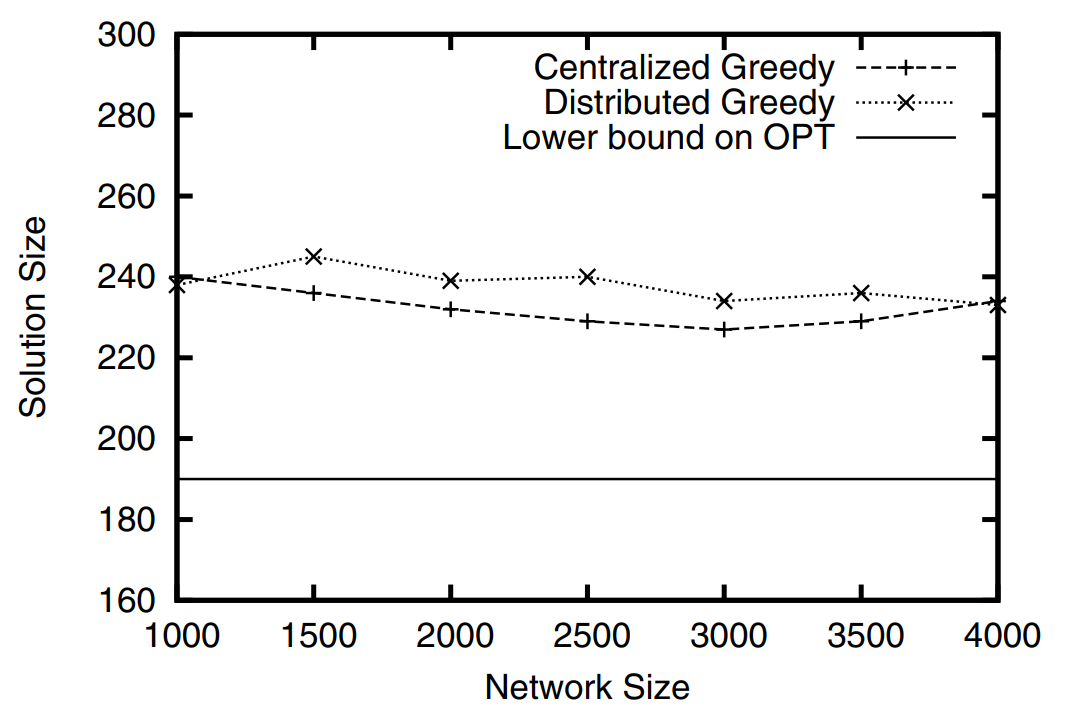
\includegraphics[width=0.7\columnwidth]{5.png}
    \caption{Solution size of 4-cover varying network size.\\ \indent Communication {radius = 4} units.}
    \label{fig:enter-label}
\end{figure}

\begin{figure}[t]
    \centering
    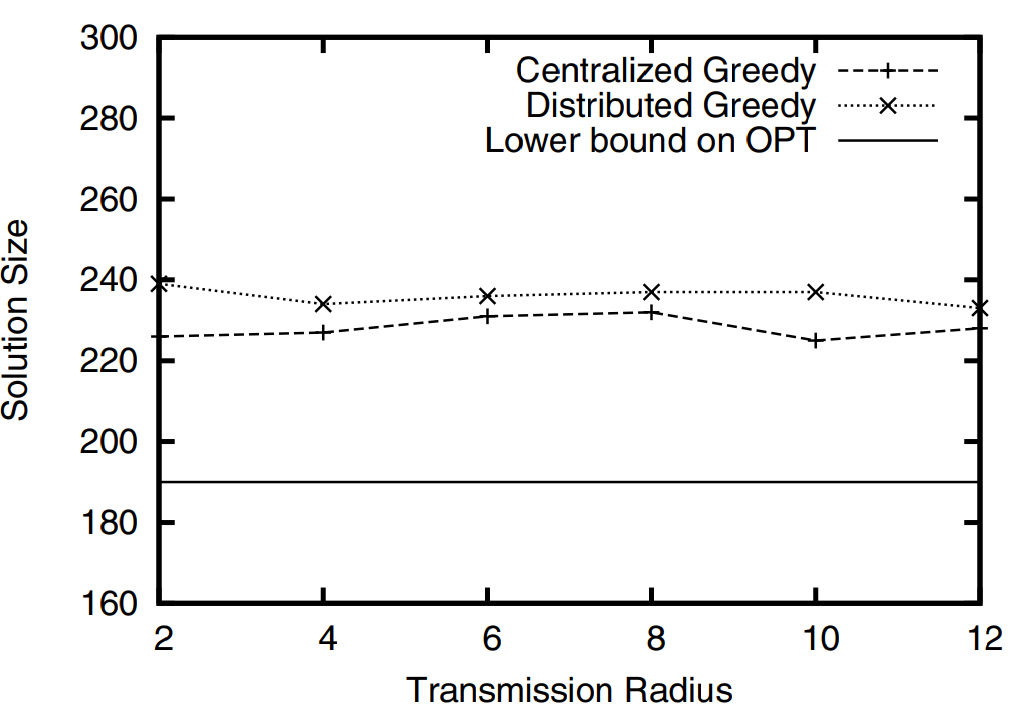
\includegraphics[width=0.7\columnwidth]{6.png}
    \caption{Solution size of 4-cover varying communication radius.\\ Sensor network size = 3000 sensors.}
    \label{fig:enter-label}
\end{figure}

\begin{theorem}
Consider an instance of Problem 3. If there exists a solution that covers $p$ percentage of the polygon area, then our greedy approach for Problem 3 gives a solution that covers at least $p/2$ percentage of the given polygon using a cost of at most $O(1/(1 - \delta) \cdot \ln \frac{p}{100}|C|)$ times the optimal cost. Here, $|C|$ is the maximum number of target points covered by a sensing regions and $\delta$ is the precision parameter.
\end{theorem}

\begin{proof_}
Let denote with $|P|$ the area of the input polygon $P$. This proof proceeds in a similar way as the proof of Theorem 1, and yields the following equation.
\begin{equation*}
    g_{j+1} \geq \frac{1-\delta}{n_{opt}}\Bigg(\frac{p}{100}|P|-2\sum_{i=1}^j g_i \Bigg)
\end{equation*}
where $g_{j+1}$ is the benefit of the sensing-region chosen in the $j^{th}$ step of the greedy approach, and $n_{opt}$ is the number of d-sensors selected by an optimal algorithm.
Note that the $(1 - \delta)$ factor is given by the use of the algorithm in [17]. Also note that after placing each d-sensor, the area that it covers should be removed from the polygon. The way to handle this situation is discussed in paragraph 2.4 of [17], and it applies to our case because the VC dimension remains 23 at each iteration of the algorithm.

By induction we can show that
\begin{equation*}
\Bigg(\frac{p}{100}|P|-2\sum_{i=1}^j g_i \Bigg) \leq \frac{p}{100} |P| \bigg(1-2\frac{1-\delta}{n_{opt}}\bigg)^j.    
\end{equation*}

Thus, when $j = n_{opt}/(2(1 - \delta)) \ln( \frac{p}{100}|P|/n_{opt})$, we have $(\frac{p}{100}|P|-2(1-\delta) \sum_{i=1}^j g_i) < n_{opt}$. Finally, observing that $n_{opt}|C|\geq|P|$ and that GA will continue until $( \frac{p}{100}|P| -2(1-\delta) \sum_{i=1}^j g_i)$ is zero, we see that when GA terminates, it has a benefit of at least $\frac{p}{100}|P|/2$ and uses at most $O(1/(1 - \delta) \cdot \ln \frac{p}{100}|C|)$ d-sensors.
\end{proof_}

\begin{theorem}
Our greedy approach for the Problem 4 gives a solution which covers at least $(1 - e^{2(1-\delta)})/2$ times the area covered by an optimal solution, for a given parameter $\delta > 0$.
\end{theorem}

\begin{proof_}
Let $M$ be the \textit{number of target points} covered by the optimal solution. This proof proceeds in a similar way as the proof of Theorem 1, and yields the following equation.
\begin{equation*}
    g_{j+1} \geq \frac{1-\delta}{n} \Bigg( M - 2 \sum_{i=1}^j g_i \Bigg)
\end{equation*}
where, $g_{j+1}$ is the benefit of the sensing-region chosen in the $j^{th}$ step of the greedy approach. Note that the $(1 - \delta)$ factor comes form the use of the approximation method of [17]. By induction, we can show that
\begin{equation*}
g_j \geq \frac{1-\delta}{n} \cdot M \cdot \bigg( 1-2\frac{1-\delta}{n} \bigg)^{j-1}
\end{equation*}
Summing all equations we get
\begin{equation*}
    \sum_{j=1}^n g_j \geq \frac{1-\delta}{n} \cdot M \cdot \sum_{j=1}^n \bigg( 1-2\frac{1-\delta}{n} \bigg)^{j-1}
\end{equation*}
which gives
\begin{equation*}
    \frac{G}{M} \geq \frac{1}{2} \bigg(1-\bigg( 1-2\frac{1-\delta}{n} \bigg)^n \bigg) \geq \frac{1}{2}\bigg( 1-\frac{1}{e^{2(1-\delta)}} \bigg)
\end{equation*}
where $G = \sum_{j=1}^n g_j$ is the total benefit of the greedy algorithm.
\end{proof_}

\section{Experimental Results}
In this section we present experimental results about the execution of GA and Distributed GA. The setup is similar to the one of [8]. Sensors are placed randomly in a square of $40 \times 40$ units. The visibility radius is set to 8, the d-sensor’s cone spans an angle of 60 degrees, and we discretize the orientations by shifts of 30 degrees. In all our experiments, $k$ is set to 4. Note that each d-sensor’s cone has an area of $8^2\pi/6$, so to 4-cover the square we need at least $4 \cdot 402 \cdot 6/(8^2\pi) \geq 190$ d-sensors.


\begin{figure}[t]
    \centering
    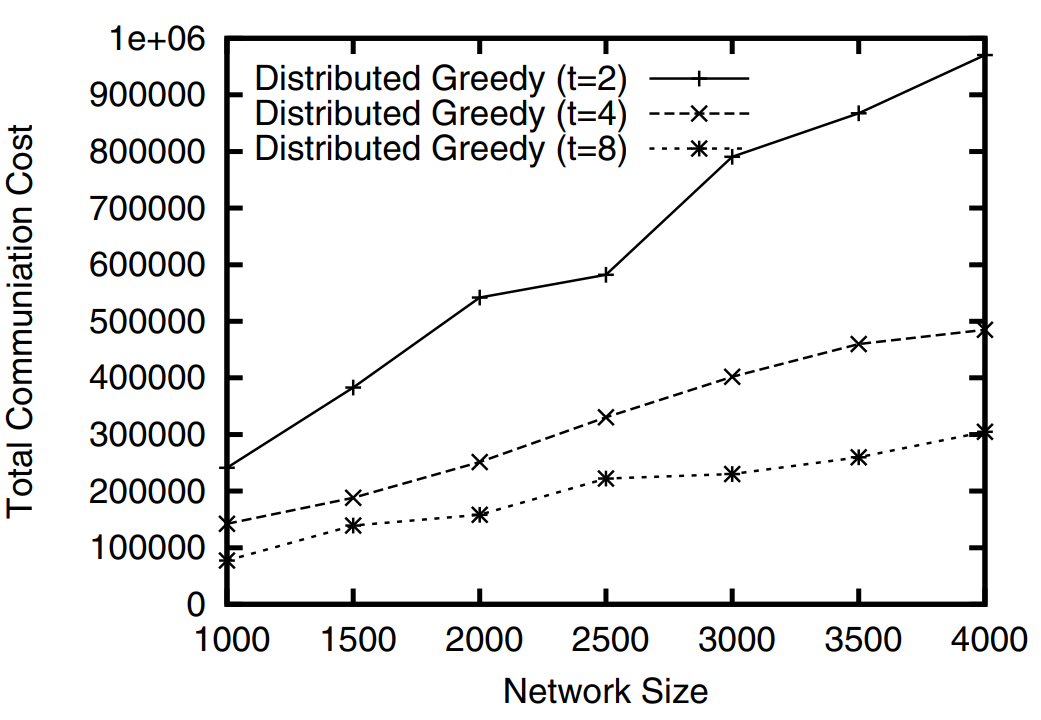
\includegraphics[width=0.7\columnwidth]{7.png}
    \caption{Communication cost of 4-cover varying the network size.}
    \label{fig:enter-label}
\end{figure}
% Communication in Distributed Algorithms. 
\begin{Communication_in_Distributed_Algorithms}
In distributed algorithms, d-sensors need to communicate with near-by d-sensors (those that cover a common target point). To reach a near-by d-sensor, a sensor broadcasts a message up to a distance $\ell$. A safe choice for $\ell$ is the \textit{link radius}, which is the maximum communication distance between any two sensors whose sensing region  intersect. We use the same methodology of [1] and [8] to compute the link radius $\ell$ of a sensor network. In particular, we define dense networks as networks with more than $r/t$ sensors within a distance $2r$, where $r$ and $t$ are the sensing and transmission radii respectively. For a $40 \times 40$ area, a dense network should have at least $(80/t)^2$ sensors, and this is the case of all our experiments. For dense networks the link radius is estimated to be $ \ell = (2r/t + 1)$.
\end{Communication_in_Distributed_Algorithms}

% Experiments. 
\begin{experiments}
In all our experiment, both GA and distributed GA were able to attain $k$-coverage (even if theoretically it is not guaranteed).
\end{experiments}

Figure 5 shows the solution size for densities that vary from 1000 to 4000, and Figure 6 shows the solution size for different communication radii. Note that 1000 sensors are barely enough to obtain 4-coverage. As the plot shows, the solution size of the greedy algorithm does not increase as the network size increases. This implies that the solution obtained for $n = 1000$ is already quite close to the optimal one. Also, note that the greedy solution is only $25\%$ higher than the theoretical lower bound on the optimal solution Moreover, the solution of Distributed GA is very close to the one of Centralized GA. This means that the method used to distribute the algorithm does not compromise much the accuracy of the solution.

Figure 7 shows how the communication cost varies for different network sizes.

% \subsection{Subsection Heading Here}
% Subsection text here.


% \subsubsection{Subsubsection Heading Here}
% Subsubsection text here.


% An example of a floating figure using the graphicx package.
% Note that \label must occur AFTER (or within) \caption.
% For figures, \caption should occur after the \includegraphics.
% Note that IEEEtran v1.7 and later has special internal code that
% is designed to preserve the operation of \label within \caption
% even when the captionsoff option is in effect. However, because
% of issues like this, it may be the safest practice to put all your
% \label just after \caption rather than within \caption{}.
%
% Reminder: the "draftcls" or "draftclsnofoot", not "draft", class
% option should be used if it is desired that the figures are to be
% displayed while in draft mode.
%
%\begin{figure}[!t]
%\centering
%\includegraphics[width=2.5in]{myfigure}
% where an .eps filename suffix will be assumed under latex, 
% and a .pdf suffix will be assumed for pdflatex; or what has been declared
% via \DeclareGraphicsExtensions.
%\caption{Simulation results for the network.}
%\label{fig_sim}
%\end{figure}

% Note that the IEEE typically puts floats only at the top, even when this
% results in a large percentage of a column being occupied by floats.


% An example of a double column floating figure using two subfigures.
% (The subfig.sty package must be loaded for this to work.)
% The subfigure \label commands are set within each subfloat command,
% and the \label for the overall figure must come after \caption.
% \hfil is used as a separator to get equal spacing.
% Watch out that the combined width of all the subfigures on a 
% line do not exceed the text width or a line break will occur.
%
%\begin{figure*}[!t]
%\centering
%\subfloat[Case I]{\includegraphics[width=2.5in]{box}%
%\label{fig_first_case}}
%\hfil
%\subfloat[Case II]{\includegraphics[width=2.5in]{box}%
%\label{fig_second_case}}
%\caption{Simulation results for the network.}
%\label{fig_sim}
%\end{figure*}
%
% Note that often IEEE papers with subfigures do not employ subfigure
% captions (using the optional argument to \subfloat[]), but instead will
% reference/describe all of them (a), (b), etc., within the main caption.
% Be aware that for subfig.sty to generate the (a), (b), etc., subfigure
% labels, the optional argument to \subfloat must be present. If a
% subcaption is not desired, just leave its contents blank,
% e.g., \subfloat[].


% An example of a floating table. Note that, for IEEE style tables, the
% \caption command should come BEFORE the table and, given that table
% captions serve much like titles, are usually capitalized except for words
% such as a, an, and, as, at, but, by, for, in, nor, of, on, or, the, to
% and up, which are usually not capitalized unless they are the first or
% last word of the caption. Table text will default to \footnotesize as
% the IEEE normally uses this smaller font for tables.
% The \label must come after \caption as always.
%
%\begin{table}[!t]
%% increase table row spacing, adjust to taste
%\renewcommand{\arraystretch}{1.3}
% if using array.sty, it might be a good idea to tweak the value of
% \extrarowheight as needed to properly center the text within the cells
%\caption{An Example of a Table}
%\label{table_example}
%\centering
%% Some packages, such as MDW tools, offer better commands for making tables
%% than the plain LaTeX2e tabular which is used here.
%\begin{tabular}{|c||c|}
%\hline
%One & Two\\
%\hline
%Three & Four\\
%\hline
%\end{tabular}
%\end{table}


% Note that the IEEE does not put floats in the very first column
% - or typically anywhere on the first page for that matter. Also,
% in-text middle ("here") positioning is typically not used, but it
% is allowed and encouraged for Computer Society conferences (but
% not Computer Society journals). Most IEEE journals/conferences use
% top floats exclusively. 
% Note that, LaTeX2e, unlike IEEE journals/conferences, places
% footnotes above bottom floats. This can be corrected via the
% \fnbelowfloat command of the stfloats package.




\section{Conclusion}
In this paper, we studied the problem of selecting and orienting a minimum number of direction sensor for $k$-coverage problem. The problem is NP-hard to approximate; however, we designed a greedy algorithm with certain performance guarantees. We designed a distributed version, and through experiments showed that the distributed implementation does not compromise much on the performance of the solution. We also addressed three other related problems that arise in the context of coverage using direction sensors, and analyze the performance of appropriate greedy approximation schemes for them.
% conference papers do not normally have an appendix


% use section* for acknowledgment
\section*{Acknowledgment}
% The authors would like to thank...
We wish to tank Prof. Joseph Mitchell for his useful
comments. The work was supported in part by NSF
Grants IIS-0713186, CNS-0721701, and CNS-0721665.





% trigger a \newpage just before the given reference
% number - used to balance the columns on the last page
% adjust value as needed - may need to be readjusted if
% the document is modified later
%\IEEEtriggeratref{8}
% The "triggered" command can be changed if desired:
%\IEEEtriggercmd{\enlargethispage{-5in}}

% references section

% can use a bibliography generated by BibTeX as a .bbl file
% BibTeX documentation can be easily obtained at:
% http://mirror.ctan.org/biblio/bibtex/contrib/doc/
% The IEEEtran BibTeX style support page is at:
% http://www.michaelshell.org/tex/ieeetran/bibtex/
%\bibliographystyle{IEEEtran}
% argument is your BibTeX string definitions and bibliography database(s)
%\bibliography{IEEEabrv,../bib/paper}
%
% <OR> manually copy in the resultant .bbl file
% set second argument of \begin to the number of references
% (used to reserve space for the reference number labels box)
% \begin{thebibliography}{100}

% \bibitem{IEEEhowto:kopka}
% H.~Kopka and P.~W. Daly, \emph{A Guide to \LaTeX}, 3rd~ed.\hskip 1em plus
%   0.5em minus 0.4em\relax Harlow, England: Addison-Wesley, 1999.
% \bibitem{ref1}H. Gupta, Z. Zhou, S. Das, and Q. Gu, "Connected sensor cover: Self-organization of sensor networks for efficient query execution," ACM/IEEE Transactions on Networking (TON), vol. 14, no. 1, 2006.

% \end{thebibliography}
% \bibliographystyle{IEEEtran}
% \bibliography{name}
% \cite{1597223}
% \cite{1146711}
% \cite{936985}
% \cite{10.1145/381677.381691}
% \cite{1181406}
% \cite{1208944}
% \cite{4215866}
% \cite{1401672}
% \cite{10.5555/40599}
% \cite{10.5555/580470}
% \cite{10.1007/BF02570718}
% \cite{10.1007/BF02187876}
% \cite{article}
% \cite{10.1145/1178782.1178800}
% \cite{10.1007/11599463_70}
% \cite{4068136}
% \cite{10.5555/982792.982954}
% \cite{Valtr1998GuardingGW}

\bibliographystyle{ieeetr}
\bibliography{name}




% that's all folks
\end{document}


